{\let\clearpage\relax\let\cleardoublepage\relax
\chapter{Disco protoplanetario}
}

Il materiale presente nella regione instabile di una nube molecolare \'e dotato di momento angolare quindi accresce sulla massa della protostella centrale formando un disco ortogonale al momento totale della nube che trascurando l'effetto della pressione del gas, ruota con velocit\'a angolare kepleriana.

\begin{workout}[Refs dischi protoplanetari]
Chronology of  early stages: apai lauretta 10 (book)
\end{workout}

\section{Modello disco di accrescimento}

Nei modelli unidimensionali per disco di accrescimento si descrive il trasporto di momento angolare verso l'esterno introducendo la viscosit\'a aumentata $\nu=\frac{\eta}{\rho}\to\alpha c_s H$: giustifico euristicamente la parametrizzazione della viscosit\'a del disco di accrescimento in analogia alla viscosit\'a molecolare (\cite{bouvier2002theory}).

\begin{workout}[Strees tensor]
appendix a pg 66 planet formation and migration vs crida PHD torque calculation pg 24
\end{workout}
\begin{workout}[Stress tensor in keplerian disk: crida PHD]
pg 26
\begin{align}
&\sigma_{ij}=d_{ij}-PI{ij}\\
&d_{ij}=2\Sigma\nu(D_{ij}-\frac{1}{3}(\div{\vec{v}}I_{ij})+\Sigma\zeta(\div{\vec{v}})I_{ij}\\
&D_{ij}=\frac{1}{2}(\partial_iv_k+\partial_kv_i)
\end{align}
\end{workout}

L'equazione del moto per un elemento di fluido
\begin{align}
&\PDof{t}(\rho v_i)+\PDof{x_i}(\rho v_iv_j+T_{ij})=F_i\\
&T_{ij}=P\delta_{ij}-\sigma_{ij}\\
&\sigma_{ij}=\eta(\partial_jv_i+\partial_iv_j-\frac{2}{3}\delta_{ij}\partial_kv_k+\zeta\delta_{ij}\partial_kv_k)
\end{align}
dove $\eta$, $\zeta$ sono le shear and bulk viscosity, quest'ultima legata ai gradi di libert\'a interni della molecola \'e trascurabile se i tempi di equipartizione interni sono molto minori del tempo fra due collisioni.
%-$\sigma_{ij}$ \'e flusso di componente i di momento in direzione j
Considero la velocit\'a istantanea di una molecola nel piano xy $(v_x+u_x,u_y)$, dove u \'e la componente casuale e $\exv{}$ rappresenta valore mediato su grande numero di particelle/tempo (agitazione termica: $\exv{u}=0$) quindi
\begin{equation}
\sigma_{xy}=-\rho\exv{u_xu_y}
\end{equation}
dove ho preso la media temporale.
D'altra parte la forza viscosa agente sulla molecola \'e
\begin{equation}
F_{visc,x}=\TDy{y}{\sigma_{xy}}\approx\TDof{y}(\eta\TDy{y}{v_x})
\end{equation}
con $\eta=\rho\nu$.
%PRIM'ORDINE IN \lambda/L
Dalle equazioni precedenti si ha che
\begin{equation}
\exv{u_iu_j}=-\nu\TDy{x_j}{v_i}
\end{equation}

Per un disco di densit\'a superficiale $\Sigma(r,t)$, dotato del campo di velocit\'a $(u_r,r\Omega+u_{\phi})$, scrivo le equazioni di conservazione di massa e la componente azimutale dell'equazione del moto
\begin{align}
&\PDy{t}{\Sigma}+\frac{1}{r}\PDof{r}(r\Sigma v_r)=0\\
&\Sigma(\PDy{t}{v_{\phi}}+v_r\PDy{r}{v_{\phi}}\frac{v_rv_{\phi}}{r})=0
\end{align}
da cui segue l'equazione del momento angolare
\begin{equation}
\PDof{t}[r\Sigma(r\Omega+u_{\phi})]+\frac{1}{r}\PDof{r}[r^2\Sigma(r\Omega+u_{\phi})u_r]=0
\end{equation}
infine, mediando le fluttuazioni su scala spaziale opportuna e trascurando la fluttuazione azimutale nel termine di derivata temporale, ottengo l'equazione
\begin{equation}
\PDof{t}r^2\Sigma\Omega+\frac{1}{r}\PDof{r}[r^3\Sigma\Omega\exv{u_r}+\Sigma r^2\exv{u_ru_{\phi}}]=0
\end{equation}
che rappresenta un fluido viscoso di velocit\'a $\vec{v}=(u_r,\Omega r)$ tensore degli stress $\sigma_{r\phi}=-\Sigma\exv{u_ru_{\phi}}$.

Nei modelli di disco di accrescimento unidimensionali si parametrizza il trasporto di momento angolare ponendo $\nu=\alpha c_s H$ dove $\alpha$ \'e parametro da fissare, $c_s$ la velocit\'a del suono e H lo spessore del disco:
\begin{equation}
\PDy{t}{\Sigma}=3\frac{1}{r}\PDof{r}[r\expy{1/2}\PDof{r}(\nu\Sigma r\expy{1/2})]\label{eq:sigmaevol}
\end{equation}

Poich\'e nei dischi protoplanetari l'autogravitazione \'e trascurabile la struttura verticale \'e determinata dalla componente lungo z dell'attrazione del corpo centrale:
%profilo termico determinato da equilibrio termico
\begin{equation}
\TDy{z}{P}=-\rho g_z=-\frac{GM_*}{r^2+z^2}sin{\theta}\rho=-\Omega^2z
\end{equation}

\begin{workout}[Profilo termico del disco]

\end{workout}

\begin{workout}[Momento torcente in disco Kepleriano]
\begin{align}
&\sigma_{ij}=2\Sigma\nu D_{ij}=\Sigma\nu\begin{pmatrix}0&-\Omega\partial_r(r\Omega)\\-\Omega+\partial_r(r\Omega)&0
\end{pmatrix}\\
\end{align}
Il momento torcente esercitato da S su $C^c$ \'e
\begin{equation}
T=\iint_{S^c}(\vec{r}\wedge\nabla\sigma)\,ds=\int_S\vec{r}\wedge(\sigma\,dl\vec{n})
\end{equation}
Nel caso S sia circonferenza di raggio r:
\begin{equation}
T_{\nu}=3\pi r^2\Omega_0\Sigma\nu
\end{equation}
\end{workout}

\begin{workout}[Passive disks]
(Refs: Ref: spectral energy distribution of T-Tauri star with passive circumstellar disk)
Dust passively reirradiate star light
\end{workout}

\begin{workout}[Struttura verticale del disco, profilo termico]
Pressione gas determinata da equilibrio idrostatico
\end{workout}

\begin{workout}[Viscous/turbulent disk]
laminar (high momentum diffusion)
mass inflow Gullbring98 \SIrange{e-9}{e-7}{\per\year}$\msun{}$
\end{workout}
\begin{workout}[MRI]
fig 10.3:
gammie 1996
\end{workout}

\begin{workout}[alpha prescription]
$\vec{v}=(u_r,r\Omega)$, stress tensor $\sigma_{r\phi}=-\Sigma\exv{u_ru_{\phi}}$.
Enhanced turbulent viscosity: $-\Sigma\exv{u_ru_{\phi}}=\Sigma\nu r\TDy{r}{\Omega}$, $\nu=v_TH$, $\alpha=v_T/c_s$
\end{workout}

\begin{workout}[Accretion disk sources]
Lodato: classical disk physics
o218, 296: disk formation, constrains from solar system
the alpha disk pg 18: theory of turbulent accretion disk
\end{workout}

\begin{workout}[Isothermal cloud collapse!]

\end{workout}

\begin{workout}[Descrizione trasporto momento angolare tramite parametrizzazione viscosit\'a]
Mass conservation + momentum conservation in viscous flow: angular momentum evolution. Phenomena: Shear viscosity - turbulence - MRI.
Nei modelli 1D per disco di accrescimento si parametrizza viscosit\'a tramite $\nu=\frac{\eta}{\rho}\to\alpha c_s H$: la viscosit\'a molecolare \'e troppo bassa  per trasportare all'esterno il momento angolare sui tempi-scala osservati.
Theory of turbulent accretion disk: pg 18, 8.
Flusso di x-momentum lungo y $\rho\exv{u_xu_y}$, dove considero la velocit\'a dell'elemento di fluido $(v_x+u_x,u_y)$ dove le $u$ rappresentano fluttuazioni della velocit\'a: $\sigma_{xy}=-\rho\exv{u_xu_y}$.
Ricordando la definizione di tensore degli stress e con $\vec{v}=v_x(y)\hat{x}$
\begin{equation}
\sigma_{ij}=\eta(\partial_jv_i+\partial_iv_j-\frac{2}{3}\delta_{ij}\partial_kv_k+\zeta\delta_{ij}\partial_kv_k \to \eta\TDy{y}{v_x}
\end{equation}
\begin{equation}
\PDof{t}(\rho v_i)+\PDof{x_i}(\rho v_iv_j+T_{ij})=F_i
\end{equation}
Fluttuazioni: $\sigma_{ij}=-\rho\exv{u_iu_j}$.
Viscosit\'a molecolare: $\exv{u_iu_j}=-\nu\TDy{x_j}{v_i}$.
Turbulence: Reynpold stress $\tau_{ij}=-\rho\exv{v_jv_i}$, $\exv{u_iu_j}=-\nu_T\TDy{x_j}{v_i}$
\begin{equation}
\PDy{t}{\Sigma}=3\frac{1}{r}\PDof{r}[r\expy{1/2}\PDof{r}(\nu\Sigma r\expy{1/2})]
\end{equation}
\end{workout}

\begin{workout}[Photoievaporation: X-EUV-FUV (Alexander13: The Dispersal of Protoplanetary Disks)]
Protoplanetary disc evolution and dispersal: the implications of X-ray photoevaporation.
\end{workout}


\begin{workout}[Foto-evaporazione]
(Photoevaporation: veras armitage 2003, Alexander13, Mordasini12. Internal/External).
EUV($E\approx13.6eV$): ionization, FUV($E\approx6-13.6eV$): dissociation, X-ray
\end{workout}

\section{YSO: distribuzione propriet\'a dischi protoplanetari}

La classificazione empirica degli young stellar object (YSO) si basa sul valore di
\begin{equation}
\alpha_{IR}=\TDly{\lambda}{\lambda F_{\lambda}}
\end{equation}
tra \SIrange{2.2}{25}{\micro\meter}.

\begin{itemize}
\item Classe 0: emissioni continua sub-millimetrica della polvere. Nubi molecolari compatte.
\item Classe 1: $\alpha_{IR}>0$ a \SI{2}{\micro\meter}.
\item Classe 2: $0\geq\alpha_{IR}\geq-1.5$. Stella T-Tauri con disco otticamente spesso a $\lambda\leq\SI{10}{\micro\meter}$.
\item Classe 3: $\alpha_{IR}\leq-1.5$. Stella T-Tauri con disco otticamente sottile a $\lambda\leq\SI{10}{\micro\meter}$.
\end{itemize}

Le condizioni iniziali delle simulazioni di popolazioni planetaria sono determinate dalle osservazioni dei dischi protoplanetari: le distribuzioni di metallicit\'a, massa, massa di polvere ed et\'a sono mostrati in ~\ref{fig:initdistro}. Il tempo caratteristico dei dischi protoplanetari, determinato misurando l'eccesso infrarosso in ammassi di et\'a diversa, \'e \SI{2.5}{\mega\year}. La massa del disco \'e ottenuta tramite fit con spettro osservato di un modello di disco.

\begin{figure}[!ht]
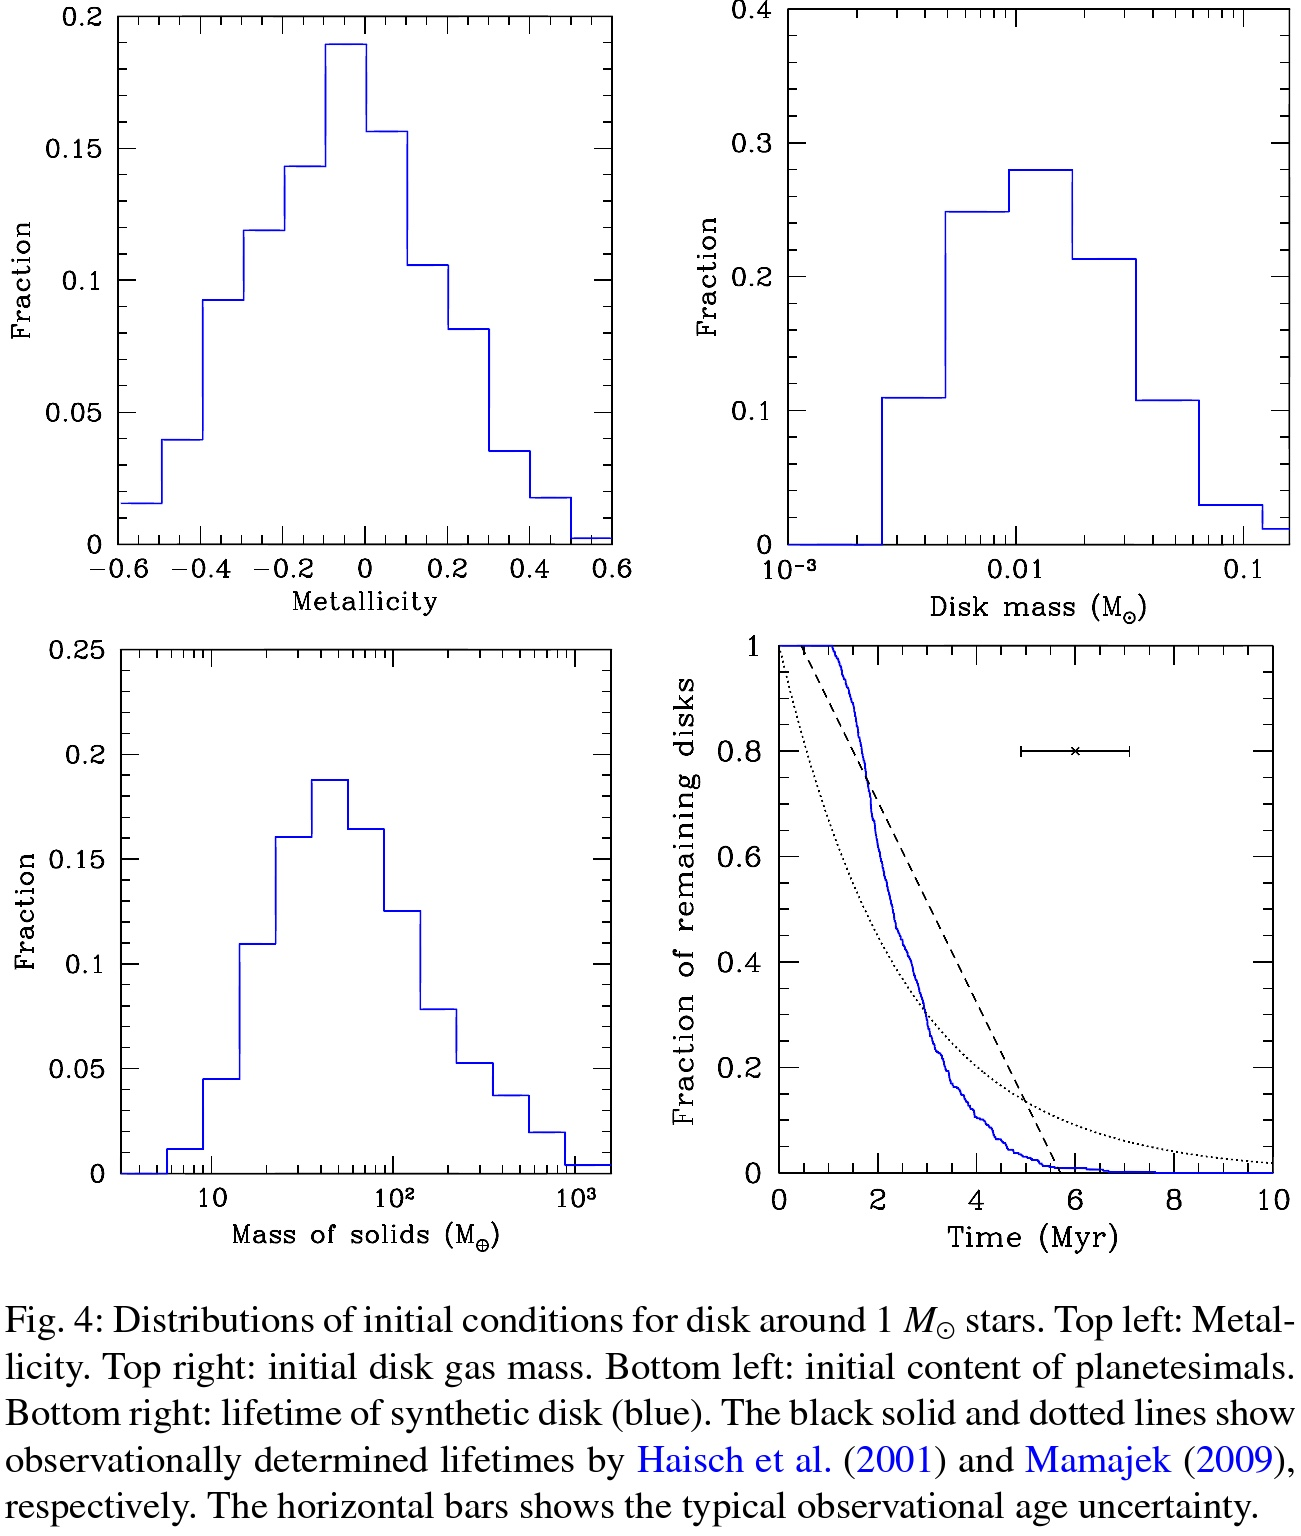
\includegraphics[trim={0cm 10cm 0 0},clip, keepaspectratio,width=0.7\textwidth]{initdistro}\label{fig:initdistro}
\caption{Distribuzione caretteristiche dischi di accrescimento. Da \cite{mordasini2018planetary}.}\end{figure}

\begin{workout}[Fit SED]
Disk model
\begin{align}
\nu\propto R\expy{\gamma}\\
\Sigma=(2-\gamma)\frac{M_d}{2\pi R_c^2}(\frac{R}{R_c})\expy{-\gamma}\\Exp{-(\frac{R}{R_c})\expy{2-\gamma}}
\end{align}
\end{workout}


\begin{workout}[Initial conditionfor protostellar collapse]
Andre 2000 - 
\end{workout}

\begin{workout}[T Tauri SED more flattish]
Ref: spectral energy distribution of T-Tauri star with passive circumstellar disk
\end{workout}

\begin{workout}[physical processes in protoplanetary disk: IRexcess, accretion rate and lifetime,]
(armitage 17): fig 1, accretion rate and lifetime (2.2 pg 5-6), inference from dust continuum (disk mass, evidence for mm-particle growth
Le stelle giovani sono caratterizzate da eccesso infrarosso fra \SIrange{2.5}{10}{\micro\meter}:
\begin{equation}
\alpha_{IR}=\TDly{\nu}{\nu F_{\nu}}
\end{equation}
Sorgenti con SED declinante in mid infrared ($2.5-10\si{\micro\meter}$): $1.5<\alpha_{IR}=<0$. Active/passive: mass infall convert G into thermalradiation/reprocessed starlight.
Refs: Perrymann 10.3 - disk formation pg 218 - 
Classification based on slope of SED between $2-25\si{\micro\meter}$: $\alpha_{IR}=\TDly{\nu}{\nu F_{\nu}}=$ (Gail Hoppo 2010)
Spitzer: forming regions within 500pc
Formation: disk quickly forms as more distant material with high angular momentum, centrifugal radius $R(t)\propto\Omega^2 t^3$: . Class 0-I : protostellar disk, gravitational unstable (cloud collapse: the collapse of the cores of slowly rotating isothermal clouds, Terebey shu cassen 1984, selfsimilar collapse of isothermal spheres and star formation, shu 77). Singular isothermal sphere: $\rho=\frac{a^2}{2\pi G}r\expy{-2}$, $M(r)=\frac{2a^2}{G}r$.
\end{workout}

\begin{workout}[disco protoplanetario: distribuzioni condizioni iniziali]

Initial disk mass
(infall phase end, no more self-gravitational instabilities) - stability(shu90), MMSN hayashi81/weidenshilling77, observations(Andrews10,Manara16) points to $(0.1-10)\%$ stellar mass, distro log-normal with mean $0.01M_*$.

{Disk lifetime}
$1-10My$ with mean $3My$ (Haisch01, Mamajek09)

\end{workout}

\begin{workout}[YSO: classificazione ]
SED: emissine a lunghezze d'onda millimetriche probano tutto il volume del disco, otticamente sottile a quelle lunghezze (Beckwith 90, Beckwith Sargent91).
$S_{\nu}\propto B_{\nu}(1-\exp{-\tau})\approx B_{\nu}\tau$: emission produced near cold disk mid-plane.
Rayleigh-jeans: $B_{\nu}\propto T$ and, since $\tau=\kappa\Sigma$, $S_{\nu}\propto \kappa\Sigma T$.
(SED: Andrews williams 07)
Survey: 0.3'', 345Ghz(870$\micro m$) 1Myr old Ophiuchus stars forming region
The absolute chronology and thermal processing of solids in the solar protoplanetary disk (Connelly Ivanova 12)
\end{workout}

\begin{workout}[Selfsimilar initial disk density solution]
Refs: Lynden-bel pringle 74
Se la viscosit\'a \'e statica e distribuita secondo $\nu\propto r\expy{\gamma}$:
\begin{align}
&R_c=R_1\mathcal{T}\expy{1/(2-\gamma)}\\
&M_d=M_{d,0}\mathcal{T}\expy{-1/2(2-\gamma)}\\
\end{align}
\end{workout}

\begin{workout}[Analitic disk model]
Chambers 09: On analytical model for the evolution of a viscous, irradiated disk
On location of snowline in protoplanetary disk (lecar chiang 06)
On the snow line in dusty PPD (Sasselov lecar 99)
Accretion disks around young object I: Detailed vertical structure (D'alessio Lizzano 98)
\end{workout}

\begin{workout}[YSO properties distro]
Refs: ''Protoplanetary Disk Structures in Ophiuchus''
da dove sono ricavete nei PPS?
mass: MMSN, andrews 10, manara 16
lifetime: IR/UV excess: haisch 01, mamajek 09
initial embryo starting position: relative spacing of few hill radii (kokubo ida 00), fill disk thinking of asyntituc isolation mass (Ida Lin 10), trapped (hasegawa pudritz 11, cridland 16)
Hueso 05: evolution of protoplanetary disk, meyer 06 Formation and evolution of planetary systems, Udry 07: statistical properties of exoplanets)
Distribuzione di probabilit\'a per condizioni iniziali.

Initial condition for planet formation (protoplanetry disk \cite{meyer2006formation}): disk metallicity, mass, lifetime, \ldots

{Metallicity and Dust/Gas}
$[M/H]$ distro modelled as normal: $\mu=-0.02$, $\sigma=0.22$ (photosphere of solar-like stars in solar neighborhood): Santos05.
$f_{dg}=f_{dg,\odot}10\expy{[M/H]}$ with $f_{dg,\odot}=0.01-0.02$.
\end{workout}

\begin{workout}[Classificazione YSO: convenzioni]
Sorgenti con SED declinante in mid infrared ($2.5-10\si{\micro\meter}$): $1.5<\alpha_{IR}=<0$. Active/passive: mass infall convert G into thermalradiation/reprocessed starlight.
Refs: Perrymann 10.3 - disk formation pg 218 - 
Classification based on slope of SED between $2-25\si{\micro\meter}$: $\alpha_{IR}=\TDly{\nu}{\nu F_{\nu}}=$ (Gail Hoppo 2010)
Spitzer: forming regions within 500pc
Formation: disk quickly forms as more distant material with high angular momentum, centrifugal radius $R(t)\propto\Omega^2 t^3$: . Class 0-I : protostellar disk, gravitational unstable (cloud collapse: the collapse of the cores of slowly rotating isothermal clouds, Terebey shu cassen 1984, selfsimilar collapse of isothermal spheres and star formation, shu 77). Singular isothermal sphere: $\rho=\frac{a^2}{2\pi G}r\expy{-2}$, $M(r)=\frac{2a^2}{G}r$
\end{workout}

\begin{workout}[Refs dischi protoplanetari]
Ciesla Dullemond10 
Perryman ch 10
williams cieza 11
Andrews 09-10
mamajek 2009 - Initial conditions of planet formation: lifetimes of primordial disks
infrared excess: gail hoppe10
\end{workout}


{\let\clearpage\relax\let\cleardoublepage\relax
\chapter{Schema di accrescimento componente solida}
}


\begin{figure}[!ht]
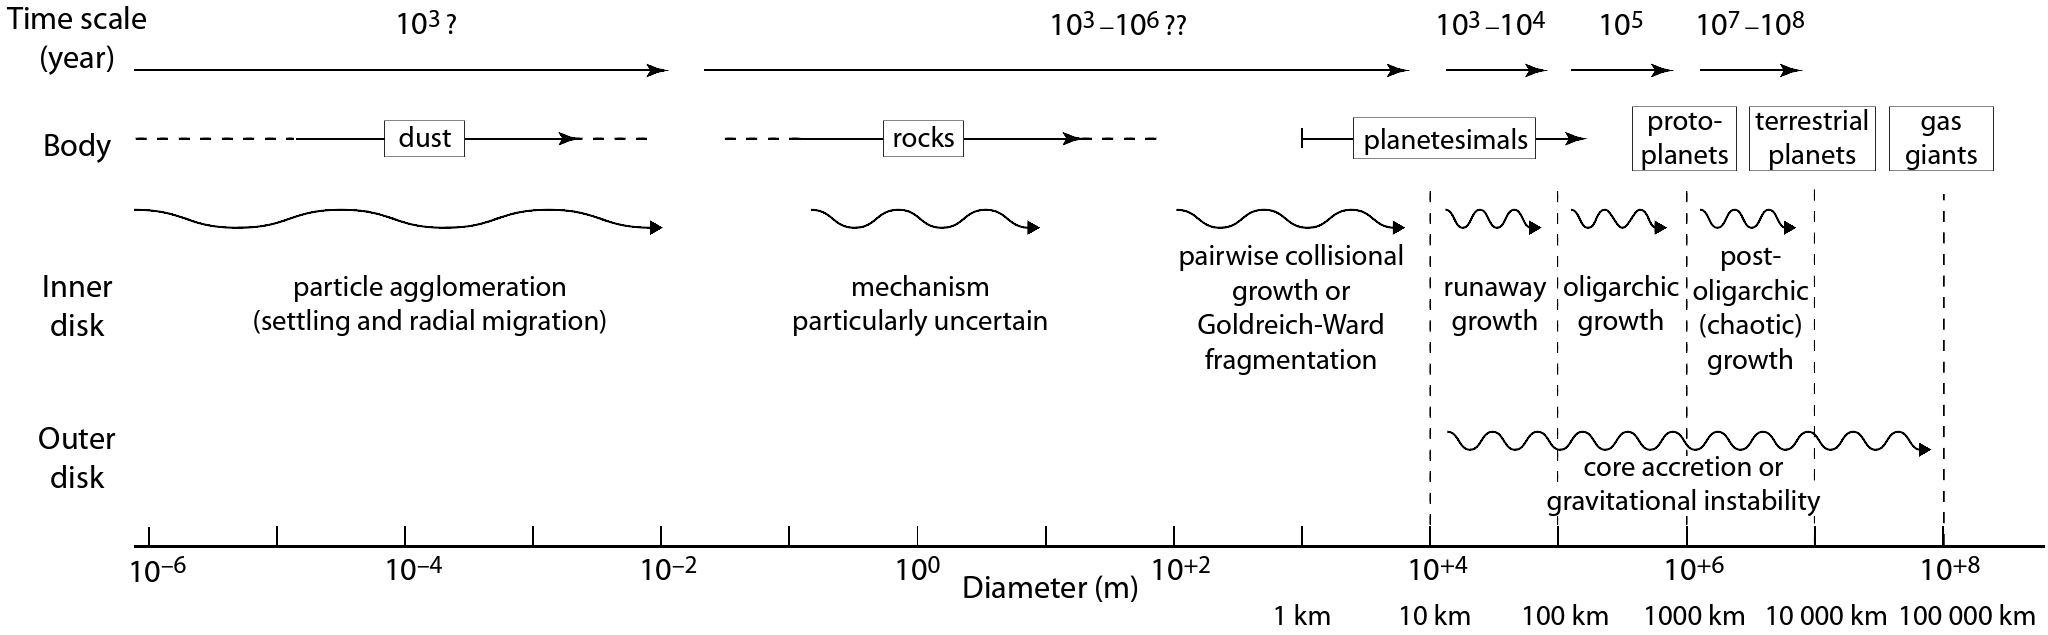
\includegraphics[width=0.9\textwidth]{accretiontimeline}\label{fig:accretiontimeline}\caption{Rappresentazione schematica del processo di formazione protopianeti dalla polvere. Da \cite{perryman2014exoplanets}.}
\end{figure}

\begin{workout}[Refs GI vs CA]
planetesimal hypoithesis: chamberlin 05, Safronov 69, Hayashi 77. Formation on dynamical scale via GI: Kuiper 51, Cameron 62.
Core accretion o instabilit\'a gravitazionale?
La correlazione tra metallicit\'a del disco protoplanetario e il numero di pianeti (giganti) \'e in accordocon osservazioni?
\end{workout}


Lo schema di core accretion (CA) prevede la coagulazione della componente polverosa in embrioni planetari che, se abbastanza massicci sono in grado di accrescere il gas presente nel disco protoplanetario.

Lo schema di formazione alternativo considera l'instabilit\'a gravitazionale del disco.

Esistono alcuni dati osservativi in favore del primo modello:
\begin{itemize}
\item arricchimento dei pianeti del sistema solare rispetto a composizione solare di metalli (la composizione di Urano/Nettuno contiene $1\%$ di $H_2$, $He$ contenuto in pianeta di composizione solare con pari massa di metalli)
\item ipotizzando una successiva rimozione della parte gassosa il pianeta deve avere il tempo di sedimentare la componente metallica
\item \'e necessario un disco di massa solare e i pianeti si formerebbero a distanza maggiore
\item non spiega la formazione dei corpi minori
\end{itemize}

\section{Sedimentazione polvere e formazione planetesimi}

La polvere presente nel materiale interstellare ha dimensioni di \SI{0.1}{\micro\meter} sedimenta verso il centro del disco e forma aggregati di dimensioni maggiori.

L'equazione del moto per particella di polvere \'e
\begin{equation}\label{eq:motiondust}
m_p\TDy{t}{v_z}=F_D-m_p\Omega^2z
\end{equation}
$F_D$ \'e la forza esercitata dal gas sulla particella di polvere
\begin{equation}
F_D=-\frac{1}{2}C_D\pi s^2\rho_gv^2
\end{equation}
nel caso cammino libero medio delle molecole di gas sia maggiore delle dimensioni della particella $C_D=\frac{8}{3}\frac{v_{th}}{v}$ (Epstein drag) per particelle pi\'u grandi \'e funzione del numero di Reynold.
%La pressione non supporta i grani: troppo pesanti

Dall'equazione \eqref{eq:motiondust} si che in condizioni stazionarie:
\begin{equation}
v_{set}=\frac{\Omega^2}{v_{th}}\frac{\rho_d}{\rho_g(z)}sz
\end{equation}
Per particelle di \SI{1}{\micro\meter} tempo di sedimentazione \'e $\SI{2e5}{\year}$.
Inoltre turbolenza e coagulazione delle particelle hanno un ruolo non banale.
%t=mv/F

La velocit\'a relativa tra gas e polvere causa un drift verso la stella massimo per particelle di \SIrange{0.01}{10}{\meter}  a \SI{1}{\astronomicalunit} per cui si deve avere rapida crescita oltre \SI{10}{\meter}.

Per passare a corpi di dimensioni kilometriche si ipotizzano 2 scenarii:
\begin{itemize}
\item La componente solida del disco di accrescimento sedimenta rapidamente in disco sottile: secondo il modello di Goldreich-Ward il disco di polvere \'e instabile e le condensazioni generano i planetesimi.
\item In assenza di sedimentazione la formazione procede tramite urti a 2 corpi e la turbolenza creando addensamenti, pu\'o accelerare la formazione di planetesimi.
\end{itemize}

\begin{workout}[refs planetesimal formation]
Armitage 07: lecture notes on formation and early evolution
 \end{workout}

\begin{workout}[Velocit\'a sedimentazione stazionaria]	
Grani piccoli raggiungono rapidamente la velocit\'a stazionaria di regime
\begin{equation}
v_{set}=\frac{\Omega^2}{v_{th}}\frac{\rho_d}{\rho_g(z)}sz
\end{equation}
 \end{workout}
 
\begin{workout}[Dust settling model]
weidenschilling 89: dust settling time
Dullemond dominique 04, johansen klahr 05, carballido 05, fromand papaloizou 06, turner 06,07
Furlan 06: Effects of dust growth and settling in T Tauri disks
Nomura 06: Dust Size Growth and Settling in a Protoplanetary Disk
\cite{lissauer1993planet}
 \end{workout}

\begin{workout}[Dust dynamics refs]
Weidenschilling cuzzi 06: Particle-gas dynamics and primary accretion, Apai Lauretta Protoplanetary Dust pg 100
Protoplanetary disk and their evolution pg 29
Protoplanetary dust: Apai Lauretta - particles dynamics pg 100
\end{workout}

\begin{workout}[Particle-gas dynamics. dust midplane sedimantation]
Weidenschilling cuzzi 06: Particle-gas dynamics and primary accretion, Apai Lauretta Protoplanetary Dust pg 100
Stopping time $t_s=\frac{\rho_sa}{\rho c_s}$ ($a<\lambda_g$). L'evoluzione dinamica delle particelle solide \'e determinata flussi macroscopici dovuti all'evoluzione del disco, gas-drag, settling
\end{workout}

\begin{workout}[Formazione planetesimi: meccanismo Goldreich-Ward]
Weidenschilling cuzzi 06: Particle-gas dynamics and primary accretion, Apai Lauretta Protoplanetary Dust pg 100
Stopping time $t_s=\frac{\rho_sa}{\rho c_s}$ ($a<\lambda_g$). L'evoluzione dinamica delle particelle solide \'e determinata flussi macroscopici dovuti all'evoluzione del disco, gas-drag, settling
\end{workout}

\section{Accrescimento planetsemi: formazione proto-pianeti.}

\subsection{Distribuzione velocit\'a planetesimi}
%Refs: kokubo Ida 12 `'Dynamics and accretion of planetesimal''
La popolazione dei planetesimi evolve attraverso interazione con gas, che smorza eccentricit\'a e inclinazione, e scattering, che trasforma il moto kepleriano in casuale.

%e si ha equipartizione di energia tra pianetesimi di diversa massa
%i planetesimi di massa minore hanno maggiore dispersione di velocit\'a 
%due planetesimi hanno stessa velocit\'a relativa prima e dopo interazione ma aumenta la velocit\'a relativa al moto kepleriano in maniera casuale: 
%\'E ragionevole supporre che si arrivi rapidamente alla condizione $v>\Omega R_H$.

%v deviazione dei planetesimi da velocit\'a kepleriana
La componente casuale della velocit\'a v dei planetesimi \'e approssimativamente
\begin{equation}
v\approx\sqrt{e^2+i^2}v_K
\end{equation}
dove si assume che eccentricit\'a e inclinazione seguano distribuzione di Rayleigh
\begin{equation}
f(e,i)=4\frac{\Sigma}{m}\frac{ei}{\exv{e^2}\exv{i^2}}\Exp{-\frac{e^2}{\exv{e^2}}-\frac{i^2}{\exv{i^2}}}
\end{equation}
I valori iniziali sono $\exv{i^2}=\exv{e^2}=[2\frac{r_H}{a}]^2$, il loro aumento, determinato da interazioni gravitazionali \'e chiamato viscous stirring, mentre , una volta formato un corpo molto pi\'u massiccio degli altri (embrione planetario), l'equipartizione di energia tra il corpo massiccio e i planetesimi produce diminuzione di eccentricit\'a/inclinazione dell'embrione planetario a scapito di aumento di queste per i corpi di massa minore.
%la velocit\'a relativa media aumenta fino al valore della velocit\'a di fuga dal corpo maggiore, denominato protopianeta raggiunto diametro migliaia di kilometri.
 
\subsection{Regimi accrescimento dei protopianeti}

L'accrescimento di massa del protopianeta procede secondo
\begin{equation}
\TDy{t}{M_e}=\pi R_c\rho_{pl}v F_g=\pi R_c\Sigma_p\Omega F_g\label{eq:Gaccretionpl}
\end{equation}
con $F_g$ fattore che tiene conto dell'interazione gravitazionale, determinato dalla velocit\'a relativa tra i 2 corpi, e $\rho_{pl}$ densit\'a di planetesimi:
\begin{align}
&\rho_{pl}\approx\frac{\Sigma_p}{2a\sin{i}}\propto\frac{\Sigma_p\Omega}{v}
\end{align}
% Costante proporzionalit\'a \'e $\frac{\sqrt{3}}{2}$ assumendo relazione di dispersione per velocit\'a planetesimi isotropa.

Per embrioni planetarii di decine di chilometri l'attrazione gravitazionale aumenta la sezione d'urto: 
\begin{equation}
\frac{1}{M_e}\TDy{t}{M_e}\propto M_e\expy{1/3}
\end{equation}
questo regime di accrescimento (runaway growth) \'e responsabile crescita diametro embrioni da \SI{10}{\kilo\meter} a \SI{100}{\kilo\meter} in \SIrange{e4}{e5}{\year}.
%(higher radial excursion ae)
Quando la massa degli embrioni domina su quella dei planetesimi si ha transizione a regime oligarchico in cui l'accrescimento \'e pi\'u lento fino a che non \'e stata accresciuta la massa presente nella zona di pertinenza gravitazionale dell'embrione,detta isolation mass,
\begin{equation}
M_{iso}\propto M_*\expy{-1/2}\Sigma_p\expy{3/2}r^3
\end{equation}

La fase finale di crescita caotica evolve il sistema verso una configurazione dinamica stabile ed ha tempi tipici di \SIrange{10}{100}{\mega\year}.

\begin{workout}[oligarchic growth rate]
La fase successiva che porta a dimensioni di migliaia di chilometri, accrescimento oligarchico ha andamento in funzione della massa
\begin{equation}
\frac{1}{M_e}\TDy{t}{M_e}\propto M_e\expy{-1/3}
\end{equation}
e tempo caratteritico $\SI{e5}{\year}$. Nel dettaglio \'e determinata 
\end{workout}

\begin{workout}[Dynamical friction]
Dynamical friction: stewart wetherill 88
\end{workout}

\begin{workout}[Dynamical evolution of planetesimal swarm: refs]
Accretional evolution of planetesimal swarm (weidenschilling 97)
Goldreich 2004: Planet Formation by Coagulation: A Focus on Uranus and Neptune
Goldreich 04: FINAL STAGES OF PLANET FORMATION
rafikov 03: DYNAMICAL EVOLUTION OF PLANETESIMALS IN PROTOPLANETARY DISKS.
rafikov 02: The growth of planetary embryos: orderly, runaway, or oligarchic?
thommes 03: Oligarchic growth of giant planets
\end{workout}

\begin{workout}[10m-10km, 100km-1000km, 1000km-10000km: refs]
Lissauer pg 142-143
Perryman pg 226
\end{workout}

\begin{workout}[Planetesimal dynamics: viscous stirring]
The origin of anisotropic velocity dispersion of particles in a disc potential (Ida, Makino 93, Stewart-Wetherill 1988 Ida1990)
\end{workout}

\begin{workout}[Gravitational stirring: Viscous stirring and dynamical friction]
\begin{itemize}
\item Viscous stirring increses i,e
\item Dynamical stirring: tends to equalize energy of random motion among bodies having different masses and velocities
\end{itemize}
\end{workout}

\begin{workout}[orbital elements distribution: rayleigh distro]
I planetesimi hanno distribuzione di velocit\'a casuale, localmente equivalente a
\begin{equation}
f(e,i)=4\frac{\sigma}{m}\frac{ei}{\exv{e^2}\exv{i^2}}\Exp{[-\frac{e^2}{\exv{e^2}}-\frac{}{\exv{i^2}}]}
\end{equation}
\'e una distro gaussiana triassiale in coordinate cilindriche (Lissauer Stewart 93)
Lissauer pg 142-143
\end{workout}

\begin{workout}[Protoplanets accretion of solids]
Other refs: Planet formation coagulation: focus on U,N (Goldreich 04), Final stages of planets formation (Goldreich 04), Formation of giant planets core: evaluating key processes (levison 09).
Safronov69: $\dot{M}_c=\Omega\Sigma_pR^2_{capture}F_G$, $R_{capture}$ larger than core radius due to gas drag, $F_G(e,i)$ gravitational focus (give rise to different growth regimes: runaway, oligarchic, orderly).
Runaway growth until protoplanets $100-1000km$ (dep on position).
Oligarchic growth: velocity of planetesimal raised by viscous stirring (gravitational scattering)/ damped by gas (until disk present).
Enhanced radius by atmospheric drag: Enhanced collisional growth of a protoplanet that has an atmosphere (Inaba Ikoma 03)
\end{workout}

\begin{workout}[orderly growth]
lissauer pg 144: equapartition effect saturation. This regime is never observed in simulations.
\begin{equation}
\frac{1}{m_p}\TDy{t}{m_p}\propto m_p\expy{-1/3}
\end{equation}
\end{workout}

\begin{workout}[runaway growth]
per planetesimi circa 1km (perch\'e?)
\begin{equation}
\frac{1}{m_p}\TDy{t}{m_p}\propto m_p\expy{1/3}
\end{equation}
\end{workout}

\begin{workout}[feeding zone: jacobi integral]
Jacobi integral
\begin{align}
&E_J=\frac{1}{2}(e^2+i^2)a^2\Omega^2-\frac{3}{8}b^2\Omega^2+\frac{9}{2}R_H^2\Omega^2\\
&\tilde{E}_J=\frac{E_J}{a^2h^2\Omega^2},\ h=R_H/a
\end{align}
Planetesimi con $\tilde{E}_J>0$ possono accrescere il protopianeta  cio\'e entro $w_{feed}=B_LR_H$, per orbite circolari $B_L=2\sqrt{3 }$.
\end{workout}

\begin{workout}[runaway to oligarchic. Isolation mass]
 NEW CONDITION FOR THE TRANSITION FROM RUNAWAY TO OLIGARCHIC GROWTH (Ormel 10)
 \begin{equation}
M_{iso}\propto M_*\expy{-1/2}\Sigma_p\expy{3/2}r^3
\end{equation}
$0.07\mearth{}$ 1AU, $9\mearth{}$ 5 AU.
Accretion among preplanetary bodies: runaway growth, summary of collision interactions
Understanding how planets become massive
\end{workout}
  
\begin{workout}[Accrescimento pianetesimi: orderly, runaway, oligarchic]
The growth of planetary embryos:  orderly, runaway, or oligarchic? (Rafikov 2002)
\begin{align}
\TDy{t}{M_e}\approx\pi R_e^2\Omega mN\frac{v}{v_z}[1+\frac{2GM_e}{R_ev^2}]
\end{align}
Accrescimento ordinato: $\frac{1}{M_e}\TDy{t}{M_e}\propto M_e\expy{-1/3}$. Accrescimento runaway: $\frac{1}{M_e}\TDy{t}{M_e}\propto M_e\expy{1/3}$. Accrescimento oligarchico: $\frac{1}{M_e}\TDy{t}{M_e}\propto M_e\expy{-1/3}$.
\end{workout}

\begin{workout}[Atmospheric drag increases accretion rate]

\end{workout}


{\let\clearpage\relax\let\cleardoublepage\relax
\chapter{Evoluzione struttura planetaria: accrescimento.}\label{chap:gasaccretion}
}% e fase isolata

Se il protopianeta raggiunge un valore critico di massa, dipendente debolmente da luminosit\'a generata da accrescimento dei pianetesimi e opacit\'a, per mantenere equilibrio idrostatico l'inviluppo gassoso del pianeta si contrae su tempi scala di Kelvin-Helmholtz.
Il flusso di massa cresce fino a esurire la massa presente nella fascia di pertinenza del protopianeta: in questa seconda fase l'accresscimento di massa \'e regolato da tempo scala viscoso del disco.

Da modelli numerici risulta
\begin{equation}
M_c^{crit}=7\mearth{}(\frac{\dot{M}_c}{\num{e-7}\mearth{}\si{\per\year}})\expy{q}(\frac{\kappa}{\SI{0.1}{\square\meter\per\kilo\gram}})\expy{s}
\end{equation}
con $q,s\approx0.2-0.3$.

\section{Accrescimento limitato da velocit\'a di raffreddamento}

La luminosit\'a del pianeta \'e determinata tramite
\begin{equation}
E_t=E_g+E_i=\int_0^M\frac{Gm}{r}\,dm+\int_{M_z}^Mu\,dm=-\xi\frac{GM^2}{2R}
\end{equation}
che sostituita nell'equazione di conservazione dell'energia da:
\begin{equation}
-\TDof{t}E_t=L=L_M+L_R+L_{\xi}=\xi\frac{GM}{R}\dot{M}-\xi\frac{GM^2}{2R^2}\dot{R}+\frac{GM^2}{2R}\dot{\xi}
\end{equation}
con $\dot{M}=\dot{M}_Z+\dot{M}_{XY}$.

Ho indicato la massa di gas legata al core con
\begin{equation}
M_{XY}=4\pi\int_{R_c}^{R_B}\rho(r')r'^2\,dr'
\end{equation}
e $R_C$ \'e il raggio del core e introduco il raggio di Bondi
\begin{equation}
R_B=G\frac{M_c}{c_0^2}\approx\SI{4e10}{\cm}a(AU)\expy{1/2}\frac{M_c}{\mearth{}}
\end{equation}
definito come raggio in cui energia termica e potenziale gravitazionale si equivalgono.%il core perturba la pressione del gas del disco.

La struttura del pianeta \'e detrminata integrando le equazioni di conservazione di massa, momento, energia e l'equazione del trasporto di energia
Mass conservation, hydrostatic equilibrium and energy transfer:
\begin{align}
&\TDy{r}{m}=4\pi r^2\rho\\
&\TDy{r}{l}=0\\
&\TDy{r}{P}=-\frac{Gm}{r^2}\rho\\
&\TDy{r}{T}=\frac{T}{P}\TDy{r}{P}\nabla(T,P)\\
&\nabla(T,P)=\TDly{P}{T}=\min{(\nad{},\nrad{})}
\end{align}


\begin{workout}[envelope mass as function of core mass]
Armitage 17 eq 232 (`'lecture nite on formation and early evolution of PS)
\begin{equation}
M_{env}\approx\int_{R_c}^{R_o}4\pi r^2\rho\,dr\propto\frac{\sigma}{\kappa_RL}(\frac{\mu m_pGM_t}{4k_b})^4\ln{\frac{R_o}{R_c}}
\end{equation}
\end{workout}

Condizioni al bordo:
\begin{align}
&R=\frac{R_A}{1+R_A/(k_lR_H )},\ P=P_{neb}\\
&\tau=\max{(\rho_{neb}\kappa_{neb}R),2/3)},\ T_i^4=\frac{3\tau L_{int}}{8\pi\sigma R^2}\\
&T^4=T_{neb}^4+T_{int}^4,\ L(R)=L_{int}
\end{align}
$k_{liss}=3-4$, quindi $R_p\approx \min{(R_B,k_{liss}\expy{-1}R_H)}$.

\begin{workout}[Hydrostatic equilibrium hypothesis]
Characterization of exoplanets from their formation I (eq 10)
\end{workout}

Rate di accrescimento limitato dalla velocit\'a di raffreddamento ($\tau\approx\tkh{}$):
\begin{equation}
\dot{M}_{XY}\propto\ \frac{M_p}{M_*}<(H_P/R_p)^3/\sqrt{3}
\end{equation}

quindi la massa di gas aumenta esponenzialmente a partire da $M_c\approx10\mearth{}$.

\section{Accrescimento limitato dalla disponibilit\'a di gas del disco}

Se $H_p\approx R_p$ il pianeta perturba in maniera non trascurabile il disco (il rate di accrescimento di gas \'e maggiore di quello fornito dal disco). Il raggio del pianeta \'e determinato dalle condizioni al bordo per materia accresciuta tramite free-fall da $R_H$ a $R_p$:
\begin{align}
&\dot{M}_{XY}=\dot{M}_{XY,max},\ v_{ff}^2=2GM(\frac{1}{R}-\frac{1}{R_H})\\
&P=P_{neb}+\frac{\dot{M}_{XY}}{4\pi r^2}v_{ff}+\frac{2g}{3\kappa},\ \tau=\max{(\rho_{neb}\kappa_{neb}R,2/3)}\\
&T_{int}^4=\frac{3\tau L_{int}}{8\pi\sigma R^2},\ T^4=(1-A)T_{neb}^4+T_{int}^4
\end{align}

In questa fase la velocit\'a di accrescimento di gas \'e determinata dall'evoluzione viscosa del disco:
\begin{equation}
\dot{M}_{e,visc}=f_{hyd}3\pi\nu\Sigma_g
\end{equation}
$f_{hyd}\approx0.9$ valore determinato da simulazioni idrodinamiche (\cite{lubow1999disk}).

\begin{workout}[Bondi accretion rate]
Unperturbed viscous flow
\begin{equation}
\dot{M}_{e,B}\approx\frac{\Sigma_g}{H}(\frac{R_H}{3})^3\Omega
\end{equation}
\end{workout}

\begin{workout}[Detached phase accretion rate]
Characterization of exoplanets from their formation pg 8
\end{workout}

\begin{workout}[Wien displacement]
$\lambda_{max}T\approx \SI{3e-3}{\meter\kelvin}$
\end{workout}

\begin{workout}[Critical core mass]
From toward deterministic
\begin{equation}
M_{c,crit}\approx10(\frac{\dot{M}_c}{\num{e-6}\mearth{}\si{\per\year}})\expy{0.2-0.3}(\frac{\kappa}{\SI{1}{\square\cm\per\gram}})\expy{0.2-0.3}\mearth{}
\end{equation}•
\end{workout}

\begin{workout}[gas accretion refs]
Lissauer 09: Models of Jupiter’s growth incorporating thermal and hydrodynamic constraints
Rafikov 10: ''Constraint on giant planet production by core accretion''
Rafikov 04 Atmospheres of protoplanetary cores: critical mass for nucleated instability.
Refs: Planet formation models: the interplay with the planetesimal disc (Fortier 2013), Characterization of exoplanets from their formation I. Models of combined planet formation and evolution (Mordasini 12)
\end{workout}

\begin{workout}[Planet-Disk exchange in hydrodynamic manner]
Ormel 15/ Cimerman 17
\end{workout}

%\section{Fase isolata}

\begin{workout}[Fase isolata: fonti energia]
fonti energia: tidal heating radiogeninc heat, star flux
\end{workout}


{\let\clearpage\relax\let\cleardoublepage\relax
\chapter{Interazioni pianeta-disco: migrazione planetaria}
}

\begin{wrapfigure}[10]{l}{0.3\textwidth}
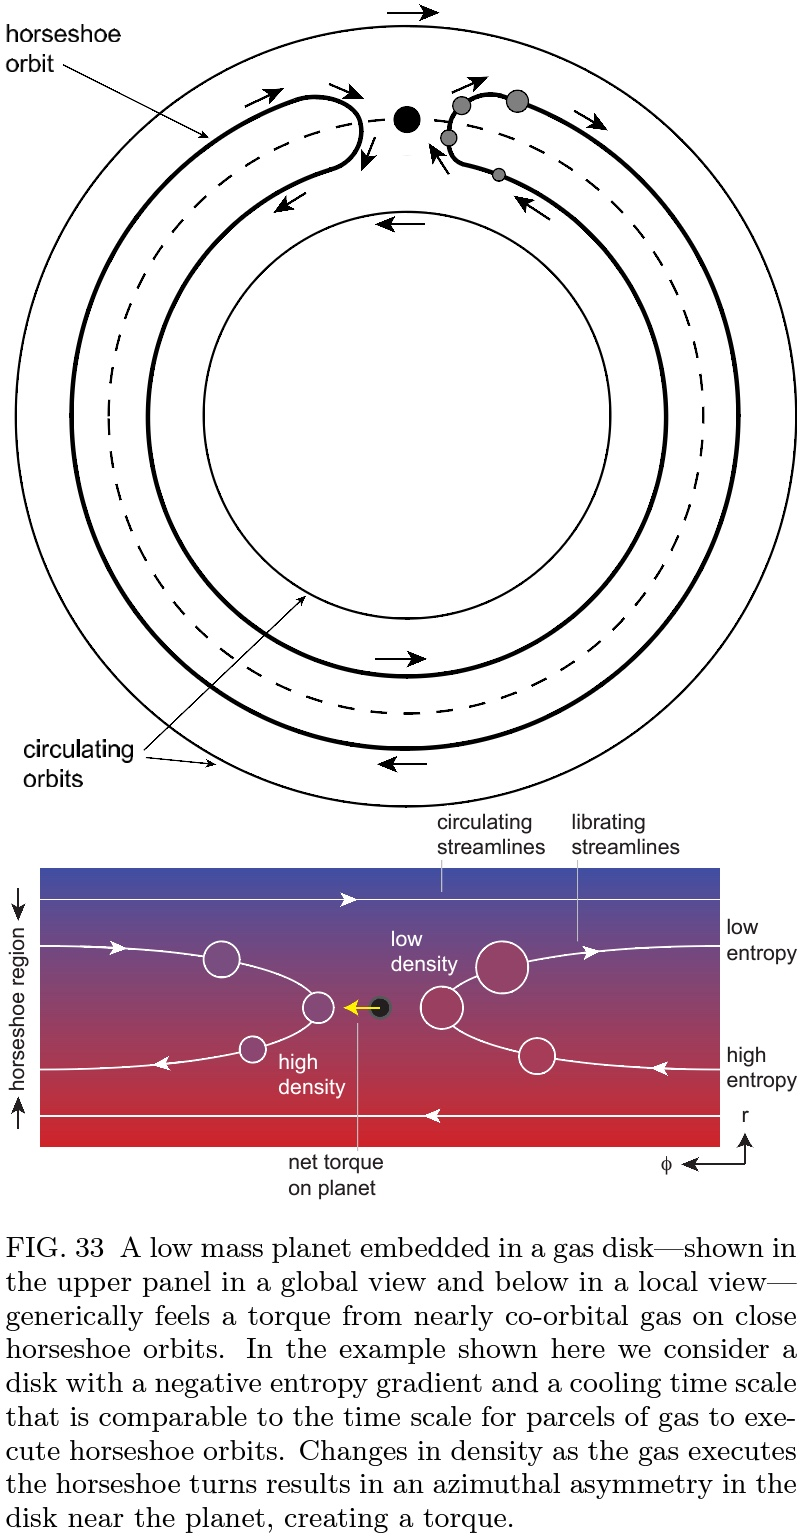
\includegraphics[trim={0cm 10cm 0 0},clip, width=0.3\textwidth]{corotation}\label{fig:corotation}
\caption{Da \cite{armitage2007lecture}.}
\end{wrapfigure}

Considero in maniera schematica lo scambio di momento angolare tra pianeta e disco usando l'approssimazione impulsiva, dove si considera la traiettora di un elemento di fluido che interagisce col pianeta e integrando sui parametri d'impatto ammissibili, oppure descrivendo in approssimazione lineare l'interazione tra onde di densit\'a e pianeta.

\clearpage

\begin{workout}[Migrazione: situazione complessa]
Armitage07 pg 57-58
\end{workout}

\begin{workout}[Migration refs]
lecture 14 (Henning Benz Klahr mordasini)
Terquem papaloizou (planet formation and migration) pg 43
Planet-disk interaction and orbital evolution
Refs: \cite{ward1997protoplanet}, \cite{terquem2000disks}, \cite{menou2004low}, (
Planet-disk interaction and orbital evolution (kley Nelson 2012), 
Baruteau 2016)
crida06: On width and shape of gaps in PPD,crida phd, 
Trilling 98:Orbital evolution and migration of giant planet: modellingextrasolar planets (Angular momentum injection rate, torque from spinning star, Impact of planet migration models on planetary populations)
Dittkrist 14: Impact of planetsmigration models n planetarypopulation (Migration II inward/outward: non equilibrium gas flow, problem of isothermal disk migration timescale: migration I regime, Fig 7;
Refs: On the tidal interaction between protoplanets and the primordial solar nebula. II - Self-consistent nonlinear interaction (1986)
Non-linear. For larger planet mass, when disk density distro is changed cons., the linear hteory is no more adeguate. If angular momentum isdeposited locally (viscous dissipation/shock waves)  the disk receeds from planets
Ida-lin04: angular momentum trasport in viscous accretion disk without planets that in type II migration act as relays that transmit angular momentum at that rateacross their gap via tidal torques.
Alibert05: the planet follow the gas except when massive than local disk.
Duffell14, Durmann kley 15: questioning that migration II follows viscous evolution of the disk but due to torque??
Planet-disk interactions: exchange of angular momentum. Low mass planet-linear theory.(''Planet-disk interactions and orbital evolution'')
Low mass planets: Lindblad and corotation torque. Rapid migration of intermediate mass planets. Gap forming massive planets: slower migration determined by viscous evolution of disk. (Role of disk self-gravity and MHD turbulence as function of planet mass).
\end{workout}

\begin{workout}[migration and disk parametrizzation]
Toward deterministic model of planetary formation IV: effects of type-I migration (highly optically thin disk)
\end{workout}

\begin{workout}[disk torque]
Orbital evolution and migration of giant planets: disk evolution and torque;
\end{workout}

\begin{workout}[Horseshoe drag refs]
Horseshoe drag in three-dimensional globally isothermal disks (masset15)
mordasini dittkrist14 (width of horseshoe region)
On horseshoe drag of a low-mass planet. I-migration in isothermal disks: relaxation of globally isothermal HP 6 (pg 29);Inroduction and first torque expression (pg1-14); 
\end{workout}

\begin{workout}[type I: migration is too fast]
magnetic fields cloud produce stocasticity and thus s migration: nelson papaloizou 04, laughlin 04
laminar/turbulent disk: nelson 05 - tidal torque on fluctuations
global magnetic fields terquem 03
global distortion (non zero eccentricity): papaloizou 02
opaciy transitionmenou goodman 04
instabilities in inviscid gap enge: koller 03
\end{workout}

\begin{workout}[planetary migration usefull formulae]
\begin{align}
\TDy{t}{j}=1/2\sqrt{GM_*/r}\TDy{t}{r}
\end{align}
Il disco di accrescimento esercita momento torcente sul pianeta che produce un trasferimento di momento angolare dal pianeta al disco $\Lambda(a,R)$
\begin{align*}
&J=M_p\sqrt{GM_*a_p}\\
&\TDy{t}{a}=2a_p\frac{\Gamma_t}{J}=-(\frac{a}{GM_*})(\frac{4\pi}{M_P})\int_{r_{int}}^{r_{out}}r\Lambda\Sigma\,dr
\end{align*}
$r_{int}, r_{out}$ inner/outer disk radius (rif to disk ar planet)
\end{workout}


\begin{workout}[M14:type I]
below few tenth of $\mearth{}$.
Linblad torque: inside/outside corotation region.
corotation torque: depends on thermodynamics regime of interaction between planet/disk.
\end{workout}

\begin{workout}[Corotation torque: non-linear (except early stages) horseshoe drag.]
(On horseshoe drag of low-mass planets)
Jump in angular momentum of particles undergoing U turn, before/after planets (in librating orbit).
ward91, masset 01,02, masset papaloizou 03, paardekooper papaloizou 09.
Linear analysis: corotation torque arise from anulus of radial extent H around corotation, launch of evanescent waves in coorbital region; horseshoe analysis consider horseshoe region.
\end{workout}

\begin{workout}[Horseshoe drag]
Horseshoe drag low-mas planet: migration in isothermal disk (casoli Masset 09): torque, width of corotation region
\end{workout}

\begin{workout}[type I: planets not massive enough to open a gap]
Linear response of disk to orbiting planets - perturbazione del pianeta sul disco si propagano come onde di densit\'a fuori dalle risonanze e come onda evanescente fra le risonanze nella regione di corotazione. Il protopianeta esercita un momento torcente sulle onde di densit\'a cha assieme  a quello di corotazione \'e responsabiledello scambio di momento angolare tra disco mkoto orbitale del pianeta: la maggior parte del toque \'e esercitato vicino alle risonanze di L./corotazione dove la lunghezza d'onda della perturbazione \'e lunga (lontano la perturbazione ha lunghezza d'onda breve: contributo mediato a zero): terquem00.
Il momento pu\'o essere calcolato facendo una analisi lineare delle onde eccitate in 2D/3D o sommando i momenti torcenti puntiformi esercitati alle risonanze di lindblad/corotazione.
\begin{align}
&t_I\propto J/\dot{J}\propto(H/a)^2\\
&t_e\propto e/\dot{e}\propto(H/a)^4
\end{align}
\end{workout}

\begin{workout}[M14:type II and outward migration]
adiabatic and local isothermal disk: pardekooper 10/11
Type II planet-dominated for mass $100\mearth{}$.
$\dot{a}_p\propto v_g$: ??
Veras armitage 04 (exoplanets with $a>20au$): outward migration seldom important, radius velocity reversal when type II migration occure $R_{mvc}$ is outside them.
\end{workout}


\section{Migrazione tipo I: pianeti piccola massa - comportamento lineare.}

\subsection{Risonanze di Lindblad}
%chapter 6 (gemelli.spacescience)
Considero un disco kepleriano ed espando il potenziale generato da un pianeta, periodico in $\phi_p=\Omega_pt$:
\begin{align}
&\psi_p(r,\phi,t)=-\frac{Gm_p}{|\vec{r}_p(t)-\vec{r}|}=\sum_{m=0}^{\infty}\psi_m(r)\cos{m[\phi-\phi_p(t)]}
\end{align}
Attorno all'orbita del pianeta si hanno orbite risonanti per elementi di fluido del gas. La condizione di risonanza \'e
\begin{align}
&\pm\kappa_0=m(\Omega-\Omega_p)\\
&r_L=(\frac{m}{m\pm1})\expy{2/3}a
%\kappa_0^2=\frac{2\Omega}{r}\TDof{r}(r^2\Omega)
\end{align}
dove $\kappa_0=\Omega$ per disco Kepleriano \'e frequenza epiciclica.

%%RMM disco pianeta: gli elementi di fluido descrivono m orbite attorno al pianeta il pianeta compie $m\pm1$ orbite

Per tenere conto della pressione introduco l'altezza scala del disco $c_s=H\Omega$. La posizione della risonanza \'e allontanata:
\begin{equation}
m[\Omega(r_L)-\Omega_p]=\mp\Omega(r_L)\sqrt{1+m^2(H/r)^2}
\end{equation}

Inoltre le risonanze rimangono a distanza finita dal pianeta:
\begin{align}
%&m(\Omega(r)-\Omega_p)=\sqrt{\kappa^2(r)(1+\xi^2)}\\
&\lim_{m\to\infty}r_L=r_p+\frac{2H}{3}
\end{align}
%dove $\xi=\frac{mc_s}{\Omega r}$, $c_s=H\Omega$.

\subsection{Momento torcente dovuto alle risonanze di Lindblad}
Il momento torcente esercitato dal disco sul pianeta \'e
\begin{equation}
\Gamma_L^{int/est}=-\int_L^{int/est}\Sigma(\vecp{r}{F})\,df=\int_L^{int/est}\Sigma(\vec{r}\wedge\nabla\psi_p)\,df=\int_L^{int/est}\Sigma\PDy{\phi}{\psi_p}\,df\label{eq:pd-torque}
\end{equation}
$\Sigma$ densit\'a superficiale,  $\vec{F}$ forza per unit\'a di massa, $df$ elemento di superficie.
%Linear. Occur if $R_H$ is smaller then H, disk scale heigth, and if viscous torque are dominant compared to gravitational torque.
(Integrando l'equazione \eqref{eq:pd-torque} si ottiene) L'espressione del momento torcente esterno/interno
\begin{equation}
%\Gamma_m^L=\left.\sign{(\Omega-\Omega_p)}\frac{\pi^2\Sigma}{3\Omega\Omega_p}(r\TDy{r}{\psi_m}+\frac{2m^2(\Omega-\Omega_p)}{\Omega}\psi_m)^2\right|_{r=r_L}
\Gamma_L^{int/est}\propto\sign{(r-r_p)}q^2\Sigma r^4\Omega^2(\frac{r}{H})^3
\end{equation}\label{eq:torqueimp}
con $q=M_p/M_*$, infine una stima del momento torcente differenziale delle risonanze di Lindblad \'e fornito da \cite{tanaka2002three}:
\begin{equation}
\Gamma_L^d\propto q^2\Sigma r_p^4\Omega_p^2(\frac{H}{r})\expy{-2}
\end{equation}
per disco isotermo infinitamente sottile.

\subsection{Momento torcente dovuto alle risonanze di Corotazione}

La regione di corotazione \'e definita da $\Omega(r)-\Omega_p=0$ cio\'e il potenziale del pianeta ruota alla stessa frequenza del fluido.

Il momento torcente dovuto alle risonanze di corotazione \'e
\begin{equation}
\Gamma_C^m\propto m[\frac{\psi_m}{\TDy{r}{\Omega}}\TDof{r}(\frac{\Sigma}{B})]_{r_c}
\end{equation}
dove $\psi_m$ \'e la m-esima componente del potenziale e $2B$ la vorticit\'a del flusso; la regione di corotazione \'e divisa in m isole di librazione.
Il gradiente di $\Sigma/B$ va rapidamente a zero se non mantenuto da adeguata viscosit\'a.
%$\nabla\wedge\vec{r}=vorticit\'a$

\subsection{Velocit\'a migrazione tipo I}

Utilizzando la stima di \cite{tanaka2002three} si trova il tempo caratteristico per migrazione tipo I

\begin{equation}
\tau_I=\frac{r_p}{|\dot{r}_p|}=\frac{\dot{J}_p}{\Gamma_{dL}}=\frac{1}{2.1+1.1\gamma}\frac{M_*}{M_p}\frac{M_*}{r_p^2\Sigma(r_p)}(\frac{c_s}{r_p\Omega_p})^2\frac{1}{\Omega_p}
\end{equation}
da cui risulta pr disco protoplanetario con $\Sigma(r)=1500(r\SI{5}{\astronomicalunit})\expy{-3/2}\si{\kilo\gram\per\square\meter}$ a $T=\SI{130}{\kelvin}$ per pianeta di massa terrestre a \SI{5}{\astronomicalunit} un tempo di migrazione $\tau_I\approx\SI{8e5}{\year}$: molto minore del tempo di vita del disco.

Il momento torcente
\begin{workout}[M14:type II and outward migration]
Freuenza epiciclica
\begin{equation}
\kappa^2=4\Omega^2+r\TDy{r}{\Omega^2}
\end{equation}
\end{workout}


\begin{workout}[Migration I in isothermal disk: pressure.]
Low mass planet in isothermal disk: linear analysis of perturbed flow.
When pressure can't be neglected the resonance condition becomes $m(\Omega(r)-\Omega_p=\sqrt{\kappa^2(r)(1+\xi^2)}$ where $\xi=\frac{mc_s}{\Omega r}$ where we used isothermal sound speed and let $c_s=H\Omega$: for $m\to\infty$ L. res position becomes $r_L=r_p+\frac{2H}{3}$ (torque cutoff).

Linear. Occur if $R_H$ is smaller then H, disk scale heigth, and if viscous torque are dominant compared to gravitational torque.
Subtypes: locally isothermal, adiabatic, un/satured-corotation torque: cooling behaviour of gas (Baruteau masset08, Casoli masset 08, paardekooper10,kley 09); timescales: dittkrist 14.
Migration timescale in isothermal approx (ida lin 08 a:):
\begin{align*}
&\tau_I=\frac{1}{2.728+1.082p_{\Sigma}}(\frac{c_s}{a_p\Omega})^2\frac{M_*}{M_p}\frac{M_*}{a_p^2\Sigma_g}\Omega\expy{-1}\\
s&\dot{a}_p=-\frac{a_p}{\tau_I}
\end{align*}
Paardekooper10, Dittkrist14: total torque $\Gamma_t=\frac{1}{\gamma}(C_0+C_1p_{\Sigma}+C_2p_T)\Gamma_0$ where $C_i$ depends upon sub-regime.
Benitez Llambay 15: heating torque, Paardekooper14 Pierens 15: dynamic corotation torque.
\end{workout}

\section{Migrazione tipo II:pianeti massicci.}

Per pianeti massicci il trasporto viscoso di momento angolare non \'e abbastanza efficiente quindi si forma un gap attorno al pianeta: questo \'e detta migrazione di tipo II. il pianeta prende momento dal disco esterno (dovuto al flusso viscoso) e cede quello richiesto al disco esterno dal trasporto viscoso: normalmente il bilancio \'e negativo quindi il pianeta migra verso l'interno.

\subsection{Approssimazione impulsiva}

%Lin papaloizou 79
\begin{wrapfigure}[14]{l}{0.45\textwidth}
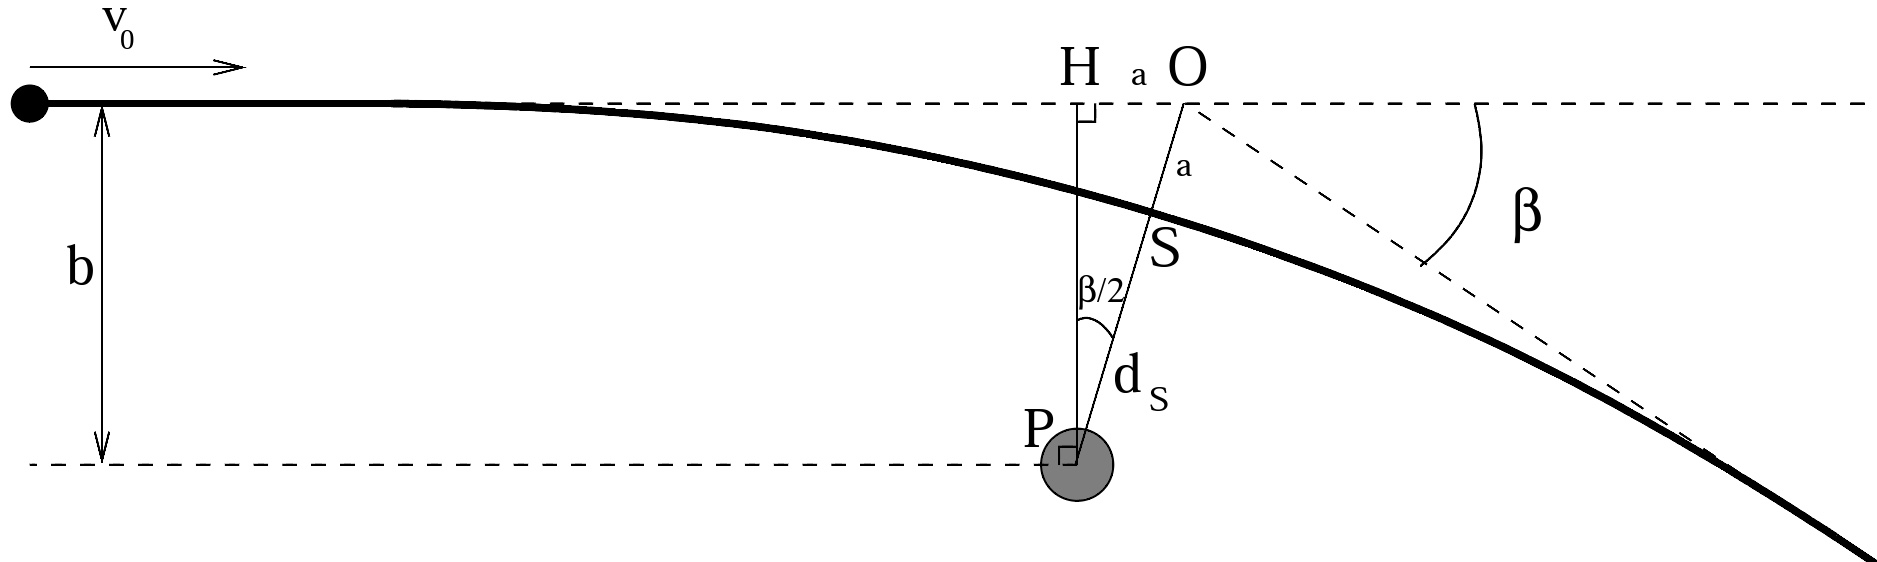
\includegraphics[width=0.45\textwidth]{impulseapprox}\label{fig:impulseapprox}
\caption{Schema approssimazione impulsiva. Da \cite{crida}.}
\end{wrapfigure}

L'approssimazione impulsiva \'e valida per incontri veloci dove la velocit\'a relativa tra elemento di fluido e pianeta \'e maggiore della velocit\'a del suono $c_s$:
\begin{equation}b_{min}=c_s|\TDy{r}{\Omega}|\expy{-1}=\frac{2}{3}H\end{equation}

In questa approssimazione posso trascurare il moto del pianeta attorno alla stella. La traiettoria di un elemento di fluido \'e deviata di un angolo
\begin{equation}
\beta=\arctan{\delta v/v}=\arctan{(\frac{GM_p}{bv_0^2})}
\end{equation}
$v_0$ velocit\'a relativa fluido-pianeta, b parametro d'impatto.

Trasferimento di momento angolareper unit\'a di massa rispetto alla stella:
\begin{align}
&v=r(\Omega-\Omega_p)\\
&\delta j=rv(\cos{\beta}-1)=-2r\frac{G^2M_p^2}{b^2v^3}
\end{align}
Il disco cede momento angolare al pianeta con rate
\begin{equation}
\frac{\delta j}{\delta t}=\frac{\delta j}{2\pi/|\Omega-\Omega_p|}
\end{equation}

Infine il momento torcente totale esercitato da pianeta sulla porzione esterna di disco che si estende da $r_p+\Delta$ a infinito \'e
\begin{equation}
\Gamma_{imp}=\int_{r_p+\Delta}^{\infty}\int_0^{2\pi}\frac{\delta j}{\delta t}\Sigma r\,d\theta\,dr\propto\Sigma q^2r_p^4\Omega_p^2\frac{r_p^3}{\Delta^3}\label{eq:torqueimp}
\end{equation}

Per materia in orbita circolare interna/esterna al pianeta il trasferimento \'e positivo/negativo: per disco esterno all'orbita l'espressione \'e la stessa con segno invertito perch\'e il disco or a \'e pi\'u lento del protopianeta.

\subsection{Regime non lineare: fromazione di gap attorno al pianeta}
%Formazione di gap per dischi tipici sopra massa di saturno.
%Viscous torque in keplerian disk: $T_{\nu}=3\pi r_0^2\Omega_0\Sigma\vu$.

Il limite del regime lineare  \'e raggiunto quando il momento torcente dovuto al potenziale del pianeta \'e pari a quello dovuto alla viscosit\'a del disco:
\begin{equation}
\Gamma_g(\Delta)+\Gamma_{\nu}(r_p+\Delta)=0
\end{equation}
con $\Gamma_g$ dato da \eqref{eq:torqueimp} o \eqref{eq:torqueimp} dove si era usata la distanza minima $\Delta=\frac{2}{3}H$.

Le condizioni necessarie per apertura gap sono (\cite{papaloizoulin1984})
\begin{align}
&R_H>H\\
&\frac{\nu}{r_p^2\Omega_p}<0.0887q^2(\frac{r_p}{H})^3
\end{align}
la prima impone che influenza gravitazionale del pianeta sia maggiore dell'altezza caratteristica del disco, la seconda che $\Gamma_g>\Gamma_{\nu}$.

\subsection{Tempi caratteristici migrazione tipo II}

Quando la massa del pianeta non eccede la massa locale del disco il tempo scale di migrazione \'e
\begin{equation}
t_{II}(yr)=\frac{1}{3\alpha}(\frac{a}{H})^2\Omega\expy{-1}=0.05/\alpha(a/H)^2(a/au)\expy{3/2}
\end{equation}
per $H/a\approx0.1$, $\alpha=\numrange{e-3}{e-2}$ a $a=1-5 au$ si ha $t_{}=10^3-10^4yr$.

\begin{workout}[approx impulsiva e regime non lineare]
(The interaction is frictional with interior speeding up protoplanet while exterior slowing down; viscous interaction with disk return mass element in circular orbit)
Il calcolo esatto che tiene conto del fatto che siamo in SR rotante (LP93) introduce fattore correttivo $K_0=4/9[2K_0(2/3)*K_1(2/3)]^2$.
La velocit\'a relativa \'e $u=a|\Omega_p-\Omega_g$ e dato che l'interazione avviene vicino al pianeta $|\Omega_p-\Omega_g|\approx3/2b\Omega_p/a$.
Rate trasferimento momento angolare tra interno del disco e pianeta
\begin{equation}
\TDy{t}{J}=\int_{b_{min}}^{+\infty}a\Sigma\Delta J|\Omega_p-\Omega_g|\,db
\end{equation}
Il parametro d'impatto minimo \'e l'assunzione implicita di un gap nel disco a assenza di materia nella regione di corotazione (discussione applicabilein regime non-lineare)
Formazione gap: perch\'e il gap si stazionario il momento scambiato nell'interazione disco-pianeta deve essere almeno quello trasportato dal moto viscoso del disco:
\begin{equation}
\TDy{t}{J}|_{visc}=3\pi\nu\Sigma a^2\omega
\end{equation}
deve essere quindi $\TDy{t}{J}|_{visc}<\TDy{t}{J}$
Cut-off: $b_{min}\approx H$, la pressione smorza effetti su scala pi\'u piccola; regime non-lneare, richiesto per gap formation, lunghezza-scala del flusso non minore di $r_H$: predndendo $b_m=2r_h$ si ha
\begin{equation}
\frac{M_p}{M_*}>\frac{40\nu}{a^2\omega}
\end{equation}
\end{workout}


\section{Migrazione tipo III}

Esistono condizioni per cui il momento torcente generato nella zona di corotazione diventa dominante.

\subsection{Momento torcente generato nella regione di corotazione}

\begin{workout}[horseshoe drag: streamline, nonlinear. corotation torque: linear]
paardekooper papaloizou 09: '' On corotation torque, horseshoe drag and the possibility of sustrained stalled or outward protoplanetary migration''.
masset 06: ''On the migration of protogiant solid cores''
\end{workout}

Il momento torcente dovuto al flusso di materia causato dalla migrazione \'e
\begin{equation}
\Gamma_{III}=2\pi\Sigma_s\dot{a}_p\Omega_pa_p^3x_s
\end{equation}

\begin{workout}[corotation torque from ''disk planet interction'']
The torque excerted by all fluid elements is (Goldreich tremaine79, Ward 91,92)
\begin{equation}
T_C3/4x_s^4\Omega_p^2\Sigma\TDly{r}{\Sigma/B}
\end{equation}
old from ''disk-planet interactions''
\begin{equation}
\Gamma_m^C=\left.\frac{m\pi^2}{2}\frac{\psi_m}{r\TDy{r}{\Omega}}\TDof{r}(\frac{\Sigma}{B})\right|_{r=r_C}
\end{equation}
$B=\frac{\kappa^2}{4\Omega}$ \'e la seconda costante di Oort (rappresenta componente z della vorticit\'a $\nabla\wedge\vec{v}|_z$).
infine il momento torcente totale \'e
\begin{equation}T_I=\sum_{m}^{int}\Gamma_m^L+\sum_{m}^{out}\Gamma_m^L+\sum_{m}\Gamma_m^C\end{equation}

Corotation torque saturation depends upon $\tau_{nlib}/\tau_{vis}$: over timescale long rel. to librration time angular momentum exchanged between planet-disk average to zero.
\end{workout}

\subsection{Corotation torque in accretion disk and migration 3 type}
Viscosity desaturate,
crida pg 39: 
Sia $b_0=r-r_p$ la distanza dal pianeta di un elemento di fluido in congiunzione
$\tau\approx2\pi/|x_s\TDy{r}{\Omega}|=4\pi r_p/(3x_s\Omega_p)$


\begin{workout}[type III and coorbital torque]
COnsidero un pianeta migrante: quando il gap \'e parziale materiale percorre l'orbita ed esercita momento t, positive/negative feedback.
Per un pianeta che migRA VERSO L'ESTERNO SI HA
$2\pi\Sigma R\TDy{t}{R}$ \'e il flusso di massa che impartisce momento per unit\'a di massa al protopianeta quando la materia attraversa la regione di corotazione di spessore w, $w\omega/2$: con $w=2H$ si ha
\begin{align}
F_{cr}=2\pi R\Sigma\omega^2 H^2\frac{1}{c_s}\TDy{t}{R}=1/2M_d\omega\TDy{t}{R}\\
F_{crb}=-1/2M_b\omega\TDy{t}{R}
\end{align}
dove la seconda \'e inerzia (??) massa legata al pianeta.
quazione del moto:
\begin{equation}
1/2M_pa\omega\TDy{t}{a}=1/2(M_d-M_b)a\omega\TDy{t}{a}+T_{ext}
\end{equation}
\end{workout}

Planet-disk interactions: exchange of angular momentum. Type III migration: planet of intermediate mass. (‘’Planet-disk interactions and orbital evolution’’).

Flow-through corotation torque: $\Gamma_{flow}=2\pi\Sigma_s\dot{a}_p\Omega_pa_p^3x_s$.

\begin{align*}
&\dot{a}_p=\frac{2\Gamma^L}{\Omega_pa_p(m_p’-\delta m)}
\end{align*}

%\section{Evoluzione elementi orbitali durante migrazione}

\begin{workout}[Eccentricity and inclination evolution]
Refs:armitage 17 ''lecturea''
Planet-disk interactions: normal, tangential, radial forces. eccentricity and inclination evolution. (‘’Planet-disk interactions and orbital evolution’’)
Decomposition of planet’s potential: non-circular orbit
\begin{align*}
&\psi_p(r,\phi,t)=-\frac{Gm_p}{|\vec{r}_p(t)-\vec{r}|}=\sum_{m=0}^{\infty}\sum_{n=-m}^m\psi_{m,n}(r)\cos{m\phi+(n-m)\Omega_pt]}
\end{align*}
Eccentricity damping.
For each m,n there are 3 resonant locations: external L resonance act to increase, corotation res. to damp (if unsaturted), and coorbital L res damp $e_p$. Linear analysis for low mass planets indicates rapid exponential damping of $e_p$:
\begin{align*}
&\TDy{t}{e_p}\propto-e_p,\ \tau_e\approx(\frac{H}{r})^2\tau_{mig}\\
&e_P>\frac{H}{r}: \TDy{t}{e_p}\propto-e_p\expy{-2}
\end{align*}
Risultati analoghi per inclinazione.	
\end{workout}


%\section{Altre interazioni che producono migrazione}


\begin{workout}[mass loss and conservation of angular momentum]
Orbital evolution and migration of giant planets: mass loss and conservation of angular momentum.
\end{workout}

\begin{workout}[torque from spinning star]
Orbital evolution and migration of giant planets: torque from spinning star
\end{workout}

\begin{workout}[planet overlflowing roche lobe migrate outward]
trilling 98:n During mass flow planet moves outward to conserve angular momentum
\end{workout}

\begin{workout}[Other (than?) types of migration]
planet-planet scattering (rasio ford 96, kozai (nagasawa 08, tidal interactions with gas disk (goldreich tremaine 80, tanaka 02))
\end{workout}

\begin{workout}[planet locked in resonances]
as solar system satellites: goldreich 65.
N-body, resonanceand migration: The dynamics of two massive planets on inclined orbits (Veras Armitage 04)
orbital migration occurring at different rates due to disk parameters can produces convergent migration and locking into mean motion resonances.
kley 04
aligned absidal line: papaloizou 03
\end{workout}


%{\let\clearpage\relax\let\cleardoublepage\relax
%\chapter{N-body interactions inside proto disk}
%}


\begin{workout}[Long-term evolution: laplace equations]
The HARPS search for southern extra-solar planets-XXVIII. Up to seven planets orbiting HD 10180: probing the architecture of low-mass planetary systems
\end{workout}
